\chapter{Experimente}
In diesem Kapitel werden wir drei verschiedenen Beispielen mit sämtliche eingeführten Methoden duchrechnen. Dabei wird zunächst auf die Lösung der Differentialgleichung eingegangen und Konvergenzbetrachtungen durchgeführt. Danach wird der Gradienten des Kostenfunktionals behandelt und die Optimierung für diverse Anfangswerte durchgeführt. %Stay Tuned!
\section{Rolling Stone}
Zum Anfang wollen wir uns dem sogenannten Rolling Stones Beispiel widmen, welches beispielsweise in \cite{boeck2014experiments} behandelt wurde. 
Es behandelt eine sich reibungslos bewegende Kugel auf einer konvexen Parabel, in dessen Mitte eine flache Ebene auf dem Intervall $[-1,1]$ eingefügt wurde. 
% [width=0.49\textwidth]
\begin{figure}[H]
% \subfigure[Bildunterschrift]{\documentclass{standalone}
\IfStandalone{
	\usepackage{pgfplots,pgfplotstable}
	\usetikzlibrary{external}
	
	}{%
}
% \usepackage{pgfplots,pgfplotstable}
% \usetikzlibrary{external}
	

\begin{document}
\tikzsetnextfilename{rolling-stones}
\begin{tikzpicture}[x=3em,y=3em]
\begin{axis}[
            xmin=-2.5,xmax=2.5,
            ymin=-1.5,ymax=1.5,
            xlabel=$z$,
%             legend entries={$V(z)$,$V'(z)$},
            width=\linewidth
        ]
        \addplot[domain=-2.5:-1]{(1+x)^2/2};
        \addplot[-,domain=-1:1]{0};
        \addplot[domain=1:2.5]{(1-x)^2/2};
        \addplot[domain=-2.5:2.5,samples=100,blue]{-min(max(-1-x,0),1-x)};
\end{axis}
\end{tikzpicture}

 
\end{document}
}\hfill
% \subfigure[Bildunterschrift]{\documentclass{standalone}
\IfStandalone{
	\usepackage{pgfplots,pgfplotstable}
	\usetikzlibrary{external}
	
	}{%
}
\begin{document}
\tikzsetnextfilename{rolling-stones-solution}
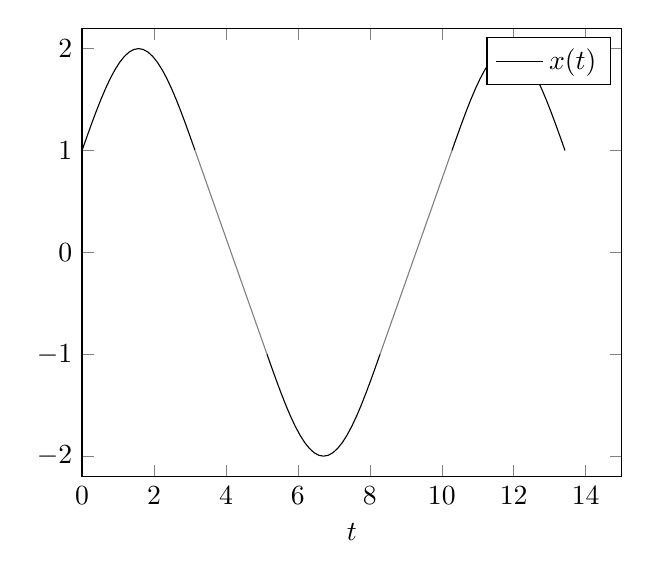
\begin{tikzpicture}[x=3em,y=3em]
\begin{axis}[
            xmin=0,xmax=15,
            ymin=-2.2,ymax=2.2,
            xlabel=$t$,
            legend entries={$x(t)$}
        ]
        \addplot[domain=0:3.14]{1+sin(deg(x))};
        \addplot[domain=pi:pi+2,gray]{1-x+pi};
        \addplot[domain=pi+2:2*pi+2]{-1-sin(deg(2-x))};
        \addplot[domain=2*pi+2:2*pi+4,gray]{x-3-2*pi};
        \addplot[domain=2*pi+4:3*pi+4]{1+sin(deg(x-2*pi-4))};
\end{axis}
\end{tikzpicture} 
\end{document}
}
\documentclass{standalone}
\IfStandalone{
	\usepackage{pgfplots,pgfplotstable}
	\usetikzlibrary{external}
	
	}{%
}
% \usepackage{pgfplots,pgfplotstable}
% \usetikzlibrary{external}
	

\begin{document}
\tikzsetnextfilename{rolling-stones}
\begin{tikzpicture}[x=3em,y=3em]
\begin{axis}[
            xmin=-2.5,xmax=2.5,
            ymin=-1.5,ymax=1.5,
            xlabel=$z$,
%             legend entries={$V(z)$,$V'(z)$},
            width=\linewidth
        ]
        \addplot[domain=-2.5:-1]{(1+x)^2/2};
        \addplot[-,domain=-1:1]{0};
        \addplot[domain=1:2.5]{(1-x)^2/2};
        \addplot[domain=-2.5:2.5,samples=100,blue]{-min(max(-1-x,0),1-x)};
\end{axis}
\end{tikzpicture}

 
\end{document}

\documentclass{standalone}
\IfStandalone{
	\usepackage{pgfplots,pgfplotstable}
	\usetikzlibrary{external}
	
	}{%
}
\begin{document}
\tikzsetnextfilename{rolling-stones-solution}
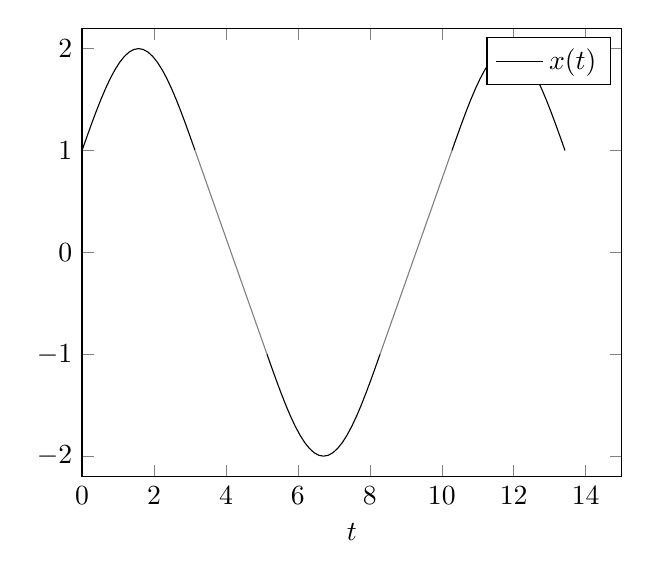
\begin{tikzpicture}[x=3em,y=3em]
\begin{axis}[
            xmin=0,xmax=15,
            ymin=-2.2,ymax=2.2,
            xlabel=$t$,
            legend entries={$x(t)$}
        ]
        \addplot[domain=0:3.14]{1+sin(deg(x))};
        \addplot[domain=pi:pi+2,gray]{1-x+pi};
        \addplot[domain=pi+2:2*pi+2]{-1-sin(deg(2-x))};
        \addplot[domain=2*pi+2:2*pi+4,gray]{x-3-2*pi};
        \addplot[domain=2*pi+4:3*pi+4]{1+sin(deg(x-2*pi-4))};
\end{axis}
\end{tikzpicture} 
\end{document}

\caption{Gesamtbild-Unterschrift}
\end{figure}


\cite{hasenfelder13}
\subsection{Problemstellung}
\subsection{Lösen der ODE}
Ode Lösung/Romberg
\subsection{Adjoints}
Plot adjoints IMP vs GIMP
\subsection{Optimierung}
Convergence
Pfad der Iterationen

\section{LC-Diode}
\cite{boeck2014experiments}
\section{Shallow Water Equation}
\subsection{Problemstellung}
\subsection{Unglattheiten}
Fluxlimiter, Eigenwerte, Plot der Rechten Seite
\subsection{Ergebnisse}


Ein oft genutztes Beispiel, um Datenassimilierungsmethoden zu testen ist die sogenannte Shallow Water Equation (vgl. \cite{zou,navon}). Diese beschreibt die Bewegung einer Flüssigkeit in einem quadratischen Gebiet unter Berücksichtigung von Gravitationswellen. In kartesischen Koordinaten erhält man folgende Gleichungen
\begin{equation}
\begin{aligned}
 \frac{\partial u }{\partial t} = -u\frac{\partial u}{\partial x} -v\frac{\partial u}{\partial y} + fv - \frac{\partial \phi}{\partial x}\\
 \frac{\partial v }{\partial t} = -u\frac{\partial v}{\partial x} -v\frac{\partial v}{\partial y} - fu - \frac{\partial \phi}{\partial y}\\
 \frac{\partial \phi }{\partial t} = -\frac{\partial u\phi}{\partial x} -\frac{\partial v\phi}{\partial y} 
\end{aligned}
\label{eq:swe}
 \end{equation}
Hierbei sind $u$ und $v$ die zwei Komponenten des Fließgeschwindigkeitsfeldes in $s^{-1}$ und $\phi$ das Geopotential in $m^2 s^{-1}$; 
$f$ bezeichnet den Coriolisfaktor.
Die Anfangsbedingungen für die folgenden Experimente wurden aus \cite{grammeltvedt}(6.I) übernommen. Es handelt sich hierbei um eine westwärtgsgerichtete Strömung mit Nord - Süd Störungen verschiedener Wellenlängen und Amplituden entlang der Zonal - Achse der Strömung. Das anfängliche Höhenfeld wurde gewählt mittels Höhenfunktion
\begin{align*}
 h(x,y) = H_0 + H_1 \tanh \left( \frac{9(y-y_0)}{2D}\right) + H_2 \sech^2\left(\frac{9(y-y_0)}{D}\right) \sin\left(\frac{2\pi x}{L}\right)
\end{align*}
und Ableitungen
\begin{align*}
 \frac{\partial h}{\partial x}(x,y) &= h_2\sech^2\left( \frac{9(y-y_0)}{D}\right) \cos\left( \frac{2\pi x}{L} \right)\frac{2\pi}{L} \\
 \frac{\partial h}{\partial y}(x,y) &= h_1 \sech^2\left( \frac{9(y-y_0)}{2D}\right)\frac{9}{2D} -  h_2\frac{18}{D} \sin\left( \frac{2\pi x}{L}\right) \frac{\sinh(9(y-y_0)/D)}{\cosh^3(9(y-y_0)/D)}\\
\end{align*}
wobei $D$ die Breite, $L$ die Länge der betrachteten Fläche ist,  $h_0 := 2000m$, $h_1 := -220m$, $h_2 := 133m$ und $y_0 = D/2$. Als schlussendliche Anfangsbedingungen ergeben sich
\begin{align*}
 \phi_0(x,y) &= gh(x,y)\\
 u_0(x,y) &= -\frac{f}{g} \frac{\partial h}{\partial y}(x,y)\\
 v_0(x,y) &= \frac{f}{g} \frac{\partial h}{\partial x}(x,y)
\end{align*}
mit $f := 10^{-4} s^{-1}$ und $g:= 10 ms^{-1}$.
Damit wir die Datenassimilierungsmethode auf (\ref{eq:swe}) anwenden können, müssen wir die Gleichung in eine Form überführen, welche nur noch von der Zeit $t$ abhängt. Grammeltvedt (in \cite{grammeltvedt}) bietet dazu diverse Finite Differenzen Schematas für die Shallow Water Equation an, mit denen sich \ref{eq:swe} in die gewünschte Form überführen lässt. In unserem Fall nutzen wir Schema F. (\ref{eq:swe}) erhält somit die Form:
\begin{equation}
 \begin{aligned}
  \frac{\partial u}{\partial t} &= -(\bar{u}^x\bar{u}^x)_x - (\bar{u}^y\bar{v}^y)_y + u(\bar{u}^x_x+ \bar{v}^y_y) +fv - \bar{\phi}^x_x\\
  \frac{\partial v}{\partial t} &= -(\bar{v}^x\bar{u}^x)_x - (\bar{v}^y\bar{v}^y)_y + v(\bar{u}^x_x+ \bar{v}^y_y) -fv - \bar{\phi}^y_y\\
  \frac{\partial \phi}{\partial t} &= -(\bar{\phi}^x\bar{u}^x)_x - (\bar{\phi}^y\bar{v}^y)_y   
 \end{aligned}
 \label{eq:schemef}
\end{equation}
mit \[
\begin{aligned}
\overline{(uv)}^x_x & = \bar{u}^{2x} \bar{v}^x_x +\bar{v}^{2x} \bar{u}^x_x \\
(\bar{u}^z\bar{v}^z)_z &= \frac{1}{2} \left[ \overline{(uv)}^x_x + u \bar{v}^x_x + v \bar{u}^x_x \right] \\
 &= \frac{1}{2} \left[ \bar{u}^{2x}\bar{v}^x_x +  \bar{v}^{2x}\bar{u}^x_x  + u \bar{v}^x_x + v \bar{u}^x_x \right]\\
 \bar{u}^x_x &= \frac{1}{\Delta} \left[ \bar{u}^x(x_i+\frac{\Delta}{2}) -\bar{u}^x(x_i-\frac{\Delta}{2})  ) \right]\\
	    &=  \frac{1}{2\Delta} \left[ u(x_i+\Delta)+u(x_i)-u(x_i)-u(x_i-\Delta) \right]\\
	    &=  \frac{1}{2\Delta} \left[ u(x_i+\Delta)-u(x_i-\Delta) \right]\\
 \bar{u}^{2x}&= \frac{1}{2} \left[ u(x_i+\Delta) + u(x_i - \Delta)\right]
\end{aligned}
\]
Mit diesen Gleichungen können wir das Schema programmieren. Die Randbedingungen sind durch starre homogene Neumannbedingungen entlang der Nord- und Süd Grenzen und periodischen Randbedingungen bezüglich der Ost/West Grenzen gegeben. Seien $x_l,x_r,y_t,y_b$ die Koordinaten bzgl. der linken (l), rechten (r), oberen (t) und unteren (b) Ränder. Dann sind die Randbedingungen folgendermaßen definiert:
\begin{equation}
 \begin{aligned}
  u(x_l,y,t) = u(x_r,y,t)\\
  v(x_l,y,t) = v(x_r,y,t)\\
  \phi(x_l,y,t) = \phi(x_r,y,t)\\
  \frac{\partial u}{\partial y}(x,y_t,t) = 0 = \frac{\partial u}{\partial y}(x,y_b,t)\\ 
  v(x,y_t,t) = 0 = v(x,y_b,t)\\
  \frac{\partial \phi}{\partial y}(x,y_t,t) = 0 = \frac{\partial \phi}{\partial y}(x,y_b,t)\\ 
 \end{aligned}
\end{equation}
